% Created 2015-03-08 Sun 13:20
\documentclass[11pt]{article}
\usepackage[utf8]{inputenc}
\usepackage[T1]{fontenc}
\usepackage{fixltx2e}
\usepackage{graphicx}
\usepackage{longtable}
\usepackage{float}
\usepackage{wrapfig}
\usepackage{rotating}
\usepackage[normalem]{ulem}
\usepackage{amsmath}
\usepackage{textcomp}
\usepackage{marvosym}
\usepackage{wasysym}
\usepackage{amssymb}
\usepackage{hyperref}
\tolerance=1000
\usepackage{minted}
\usepackage{color}
\usepackage{listings}
\usepackage{algorithmic}
\usepackage{mathtools}
\author{Xiaolong Zhang}
\date{2015-01-16 Fri}
\title{Stanford Machine Learning Notes}
\hypersetup{
  pdfkeywords={Machine Learning,notes},
  pdfsubject={This is the notes when I'm learning Stanford Machine Learning on Coursera},
  pdfcreator={Emacs 24.4.1 (Org mode 8.2.10)}}
\begin{document}

\maketitle
\section*{Info}
\label{sec-1}
URL is \url{https://class.coursera.org/ml-005/lecture}

\section*{Introduciton}
\label{sec-2}
\subsection*{What is machine learning}
\label{sec-2-1}
\begin{itemize}
\item Arthur Samuel (1959): \textbf{Field of study of that gives computers the ability to learn without being explicitly programmed.}
\item Tom Mitchel (1998): A Well-posed Learning Problem is *A computer program is said to learn from experience E with repsect to some task T and some performance measure P, if its performance on T, as measured by P, improves with experience E.
\end{itemize}
\subsection*{Machine learning algorithms:}
\label{sec-2-2}
We mainly talks about \textbf{two types of algorithm}:
\begin{itemize}
\item Supervised Learning
\item Unsupervised Learning
\item Others: Reinforcement Learning, Recommender System.
\end{itemize}
And \textbf{Practical advice for applying learning algorithm}
\subsubsection*{Supervised Learning}
\label{sec-2-2-1}
"Right Answers" are given. 
\begin{itemize}
\item Regression (Housing price prediction)
\label{sec-2-2-1-1}
Predict continuous valued output (price)
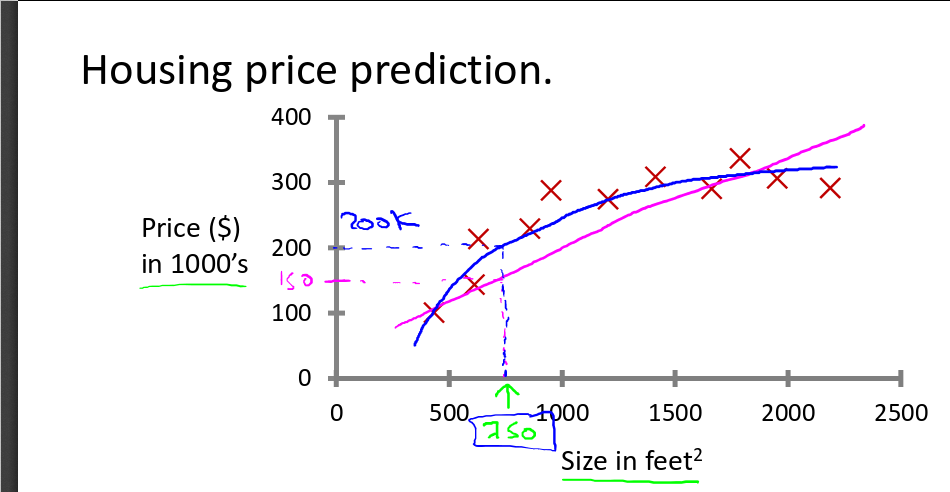
\includegraphics[width=.9\linewidth]{./images/screenshot-01.png}
\item Classification (Breast cancer (malignant, benign)
\label{sec-2-2-1-2}
Discrete valued output (0 or 1)
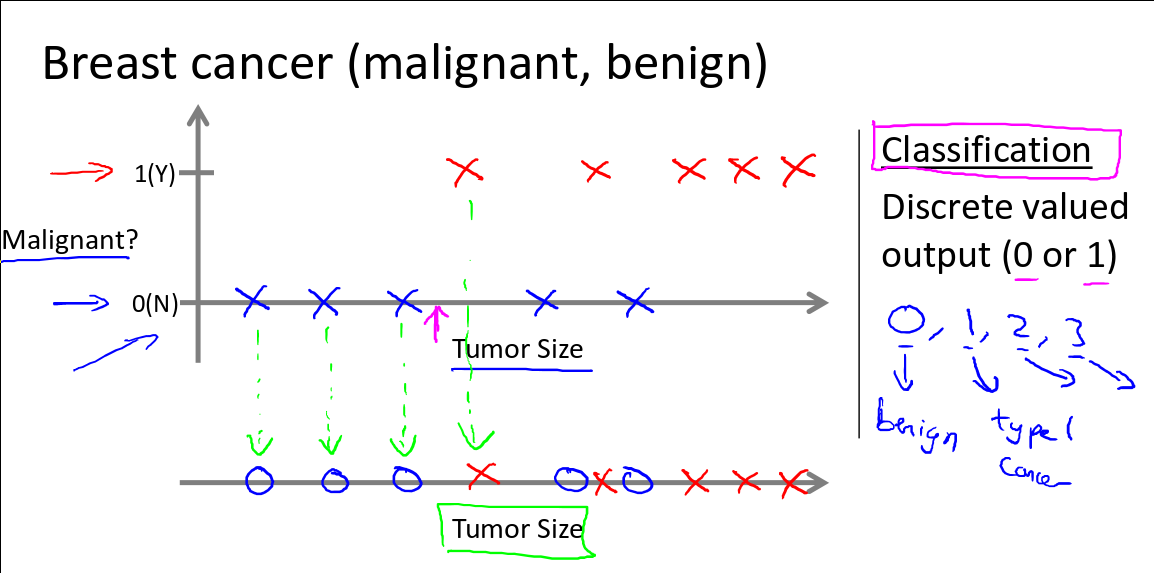
\includegraphics[width=.9\linewidth]{./images/screenshot-02.png}
\end{itemize}

\subsubsection*{Unsupervised Learning}
\label{sec-2-2-2}
No knowledge is given.
\begin{itemize}
\item Google News Grouping
\label{sec-2-2-2-1}
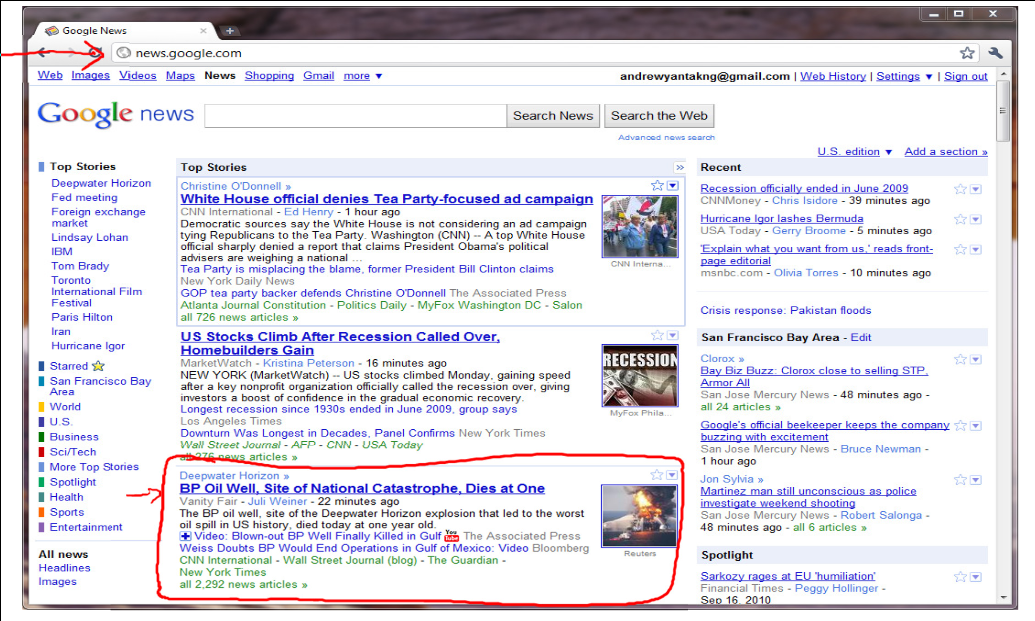
\includegraphics[width=.9\linewidth]{./images/screenshot-03.png}
\item Cocktail party problem
\label{sec-2-2-2-2}
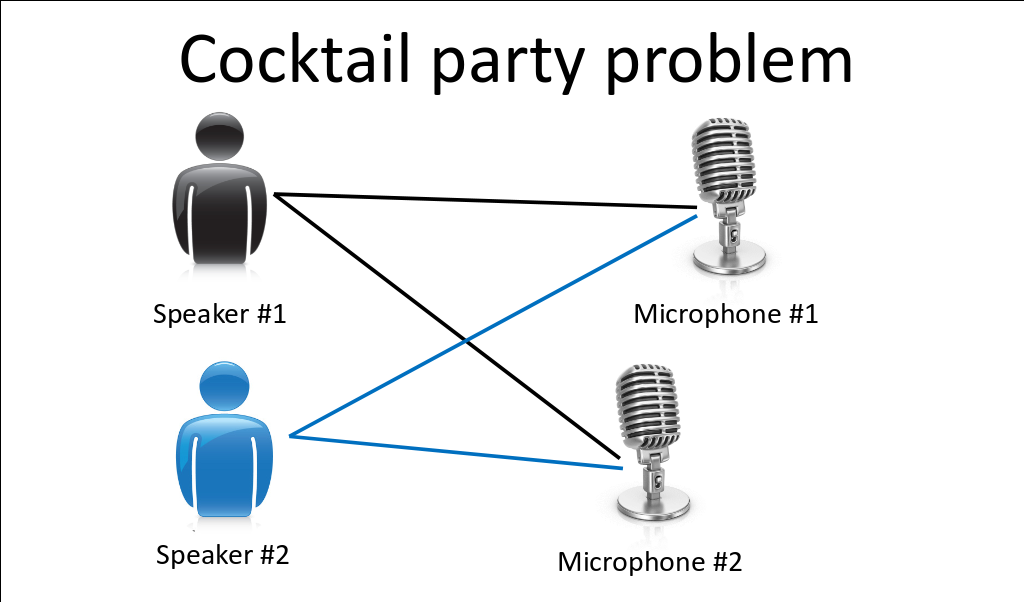
\includegraphics[width=.9\linewidth]{./images/screenshot-04.png}
\end{itemize}
\section*{Linear Regression (Week 1)}
\label{sec-3}
\subsection*{Model Representation}
\label{sec-3-1}
Notations:
\begin{enumerate}
\item \(m\) is Number of training examples.
\item \(x\)'s is "input" variable  / feature.
\item \(y\)'s is "output" variable / "target" variables.
\item \((x,y)\) is one training example.
\item \((x^{(i)},y^{(i)})\) is the \(i\)th example, \(i\) starts from \(0\).
\item \(h\) is called hypothesis, it maps the input to output. In this lecture, we represent \(h\) using linear function, thus it's called \textbf{linear regression}. For linear regression with one variable, it's called \textbf{univariate linear regression}. For example, the \textbf{univariate linear regression} is usually written as: \(h_\theta (x) = \theta_0 + \theta_1 x\). The \(\theta\) here represents the coefficient variables. Sometimes it's written as \(h(x)\) as a shorthand.
\end{enumerate}
\subsection*{Cost Function}
\label{sec-3-2}
Since the hypothesis is written as \(h_\theta (x) = \theta_0 + \theta_1 x\), where \(\theta_i\)'s are the parameters, then how to choose \(\theta_i\)'s?
The idea is to choose \(\theta_0, \theta_1\) so that \(h_\theta (x)\) is close to \(y\) for our training examples \((x,y)\). More formally, we want to
\[
\underset{\theta_0,\theta_1}{\text{minimize}} \frac{1}{2m}\sum_{i=1}^{m}\left( h_\theta(x^{(i)}) - y^{(i)} \right)^2
\],
where \(m\) is the number of trainnig examples. To recap, we're minimizing half of the averaging error. Note that the variable here are \(\theta\)s, and \(x\) and \(y\)'s are constants.

By convention, we define the \textbf{cost function} \(J(\theta_0,\theta_1)\) to represent the objective function. That is
\begin{gather*}
J(\theta_0,\theta_1) = \frac{1}{2m}\sum_{i=1}^{m}\left( h_\theta(x^{(i)}) - y^{(i)} \right)^2 \\
\underset{\theta_0,\theta_1}{\text{minimize}} J(\theta_0,\theta_1)
\end{gather*}

This cost function is also called \textbf{squared error function}. There are other cost functions, but it turns out that squared error function is a resonable choice and will work for most of regression problem.
\subsection*{Cost Function Intuition}
\label{sec-3-3}
Before getting a intuition about the cost function, let's have a recap, we now have
\begin{enumerate}
\item Hypothesis: \[h_\theta (x) = \theta_0 + \theta_1 x\]
\item Parameters: \[\theta_0,\theta_1\]
\item Cost Function: \[J(\theta_0,\theta_1) = \frac{1}{2m}\sum_{i=1}^{m}\left( h_\theta(x^{(i)}) - y^{(i)} \right)^2 \]
\item Goal: \[\underset{\theta_0,\theta_1}{\text{minimize}} J(\theta_0,\theta_1)\]
\end{enumerate}

In order to visualize our cost function, we use a simplified hypothesis function: \(h_\theta (x) = \theta_1 x\), which sets \(\theta_0\) to \(0\). So now we have
\begin{enumerate}
\item Hypothesis: \[h_\theta (x) =  \theta_1 x\]
\item Parameters: \[\theta_1\]
\item Cost Function: \[J(\theta_1) = \frac{1}{2m}\sum_{i=1}^{m}\left( h_\theta(x^{(i)}) - y^{(i)} \right)^2 \]
\item Goal: \[\underset{\theta_1}{\text{minimize}} J(\theta_1)\]
\end{enumerate}

So now let's compare function \(h_\theta (x)\) and function \(J(\theta_1)\):
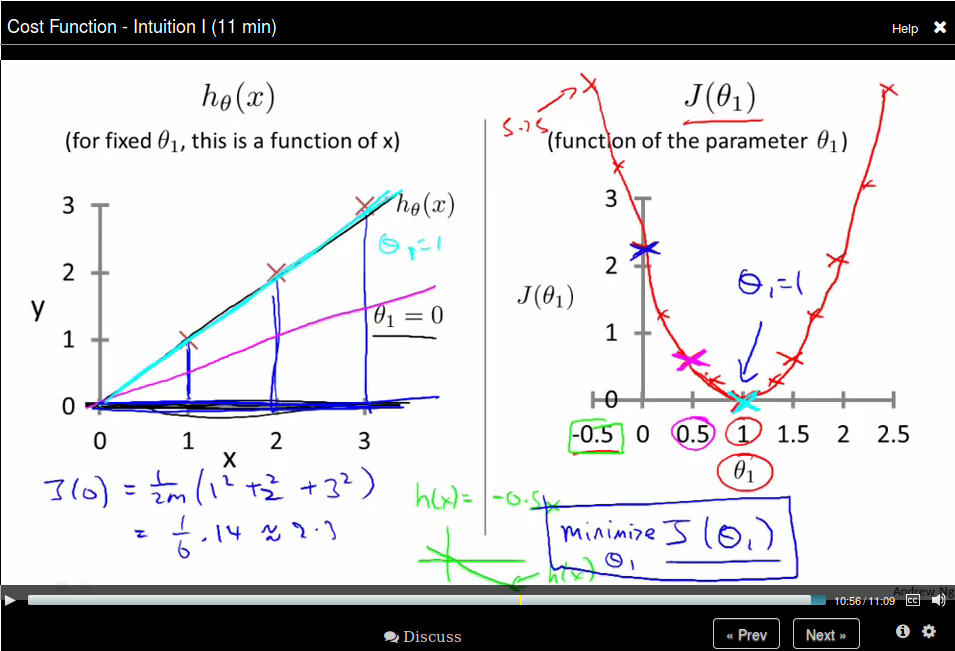
\includegraphics[width=.9\linewidth]{./images/screenshot-05.png}

Then let's come back to the original function, where we don't have the constrain that \(\theta_0 = 0\). The comparison is like
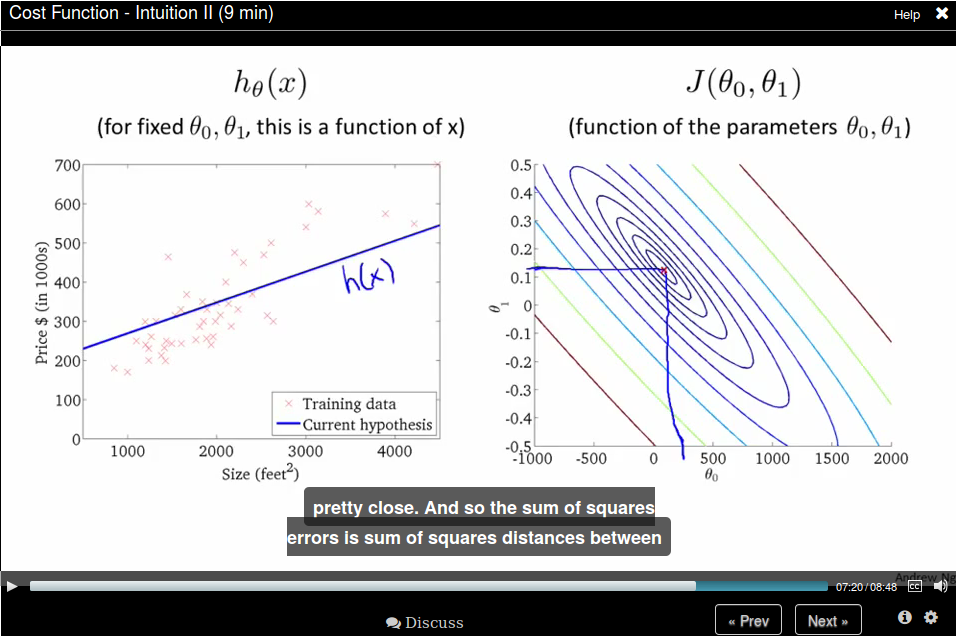
\includegraphics[width=.9\linewidth]{./images/screenshot-06.png}
\subsection*{Gradient Descent}
\label{sec-3-4}
Now we have some function \(J(\theta_0,\theta_1)\) and we want to \(\underset{\theta_0,\theta_1}{\text{minimize}}J(\theta_0,\theta_1)\), we use \textbf{gradient descent} here, which
\begin{enumerate}
\item Start with some \(\theta_0,\theta_1\),
\item Keep changing \(\theta_0,\theta_1\) to reduce \(J(\theta_0,\theta_1)\), until we hopefully end up at a minimum.
\end{enumerate}

To help understand gradient descent, suppose you are standing at one point on the hill, and you want to take a small step to step downhill as quickly as possible, then you would choose the deepest direction to downhill.
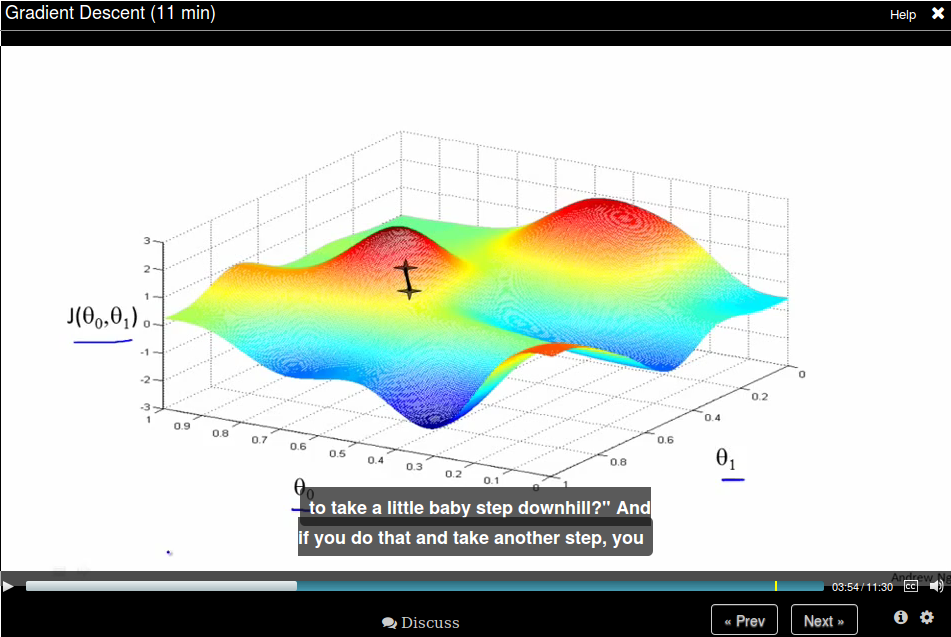
\includegraphics[width=.9\linewidth]{./images/screenshot-07.png}
You keep doing this until to get to a local minimum.
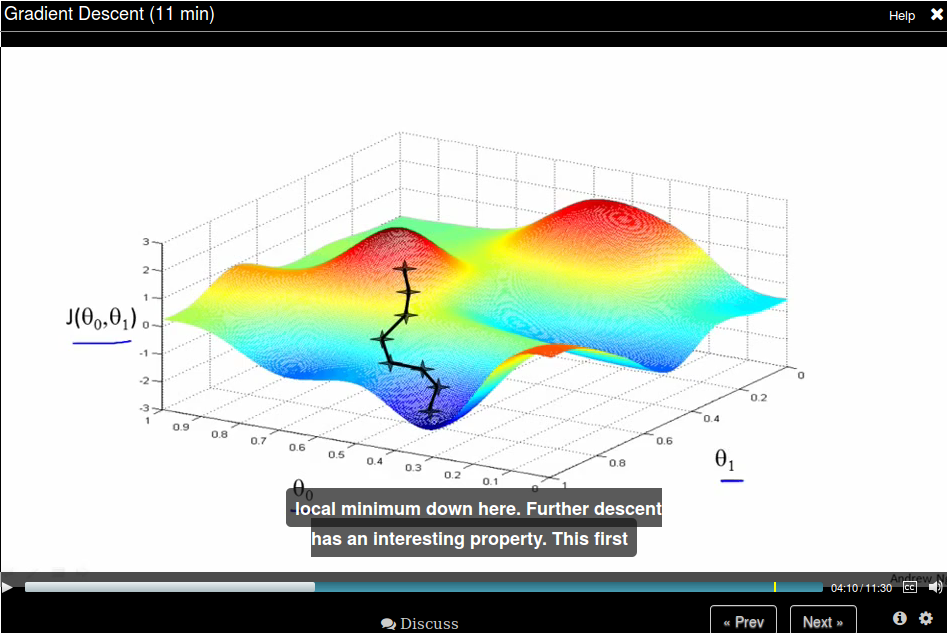
\includegraphics[width=.9\linewidth]{./images/screenshot-08.png}

But if you start with a different initial position, gradient descent will take you to a (very) different position.
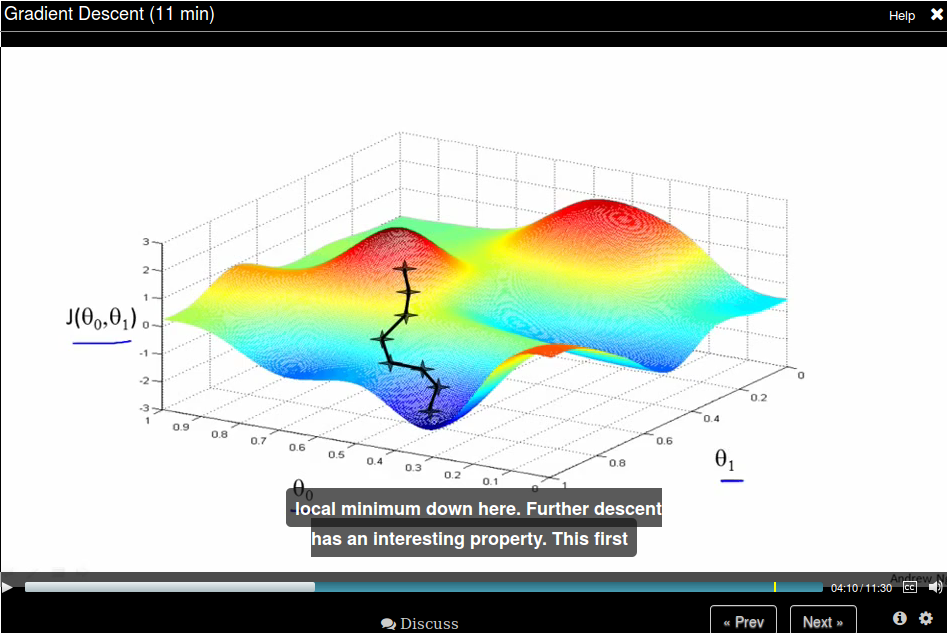
\includegraphics[width=.9\linewidth]{./images/screenshot-08.png}
\subsubsection*{Gradient Descent algorithm}
\label{sec-3-4-1}

We use $a := b$ to represent \textbf{assignment} and \( a = b\) to represent \textbf{truth assertion}.



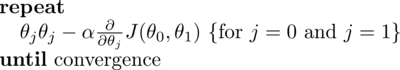
\includegraphics[width=.9\linewidth]{test.png}


The $\alpha$ here is called learning rate.

Pay attention that when implementing gradient descent, we need to update all $\theta\text{s}$ simultaneous.
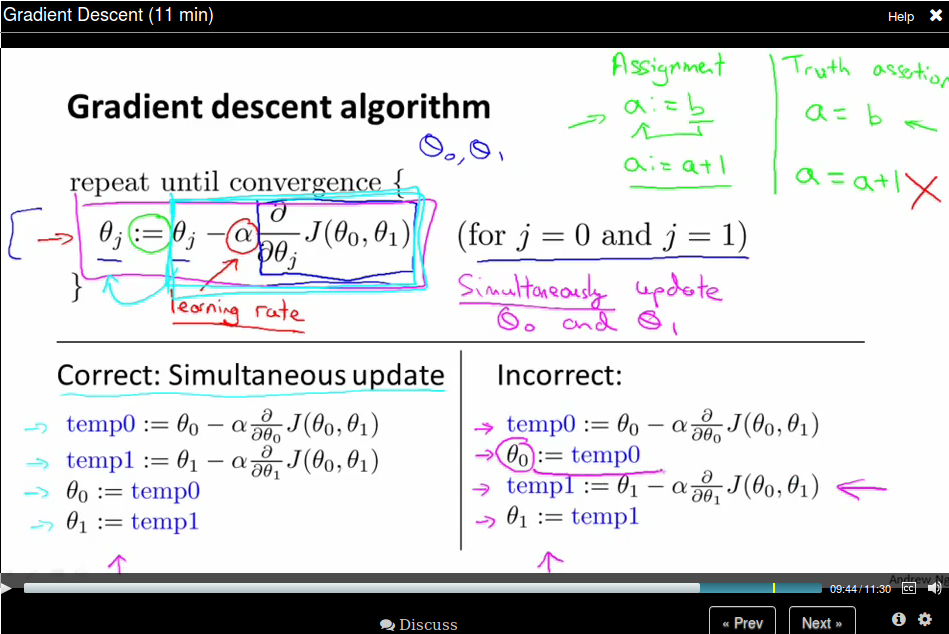
\includegraphics[width=.9\linewidth]{./images/screenshot-10.png}

Recall that $\alpha$ is a called the learning rate, which is actually a scale factor to our step represented by the derivative term. Take a 1D case as an example, the derivative is the direction (slop of the tanget line) where the function value becomes larger, so we should take its negative as our step.
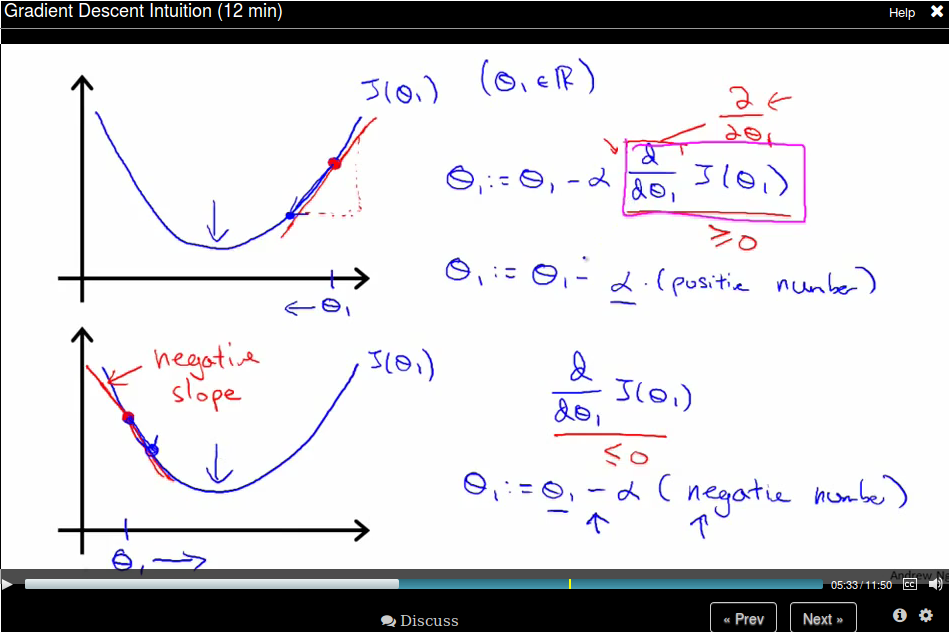
\includegraphics[width=.9\linewidth]{./images/screenshot-11.png}


If $\alpha$ is too small, gradient descent can be slow. If $\alpha$ is too large, gradient can overshoot the minimum. It may fail to converge, or even diverge.
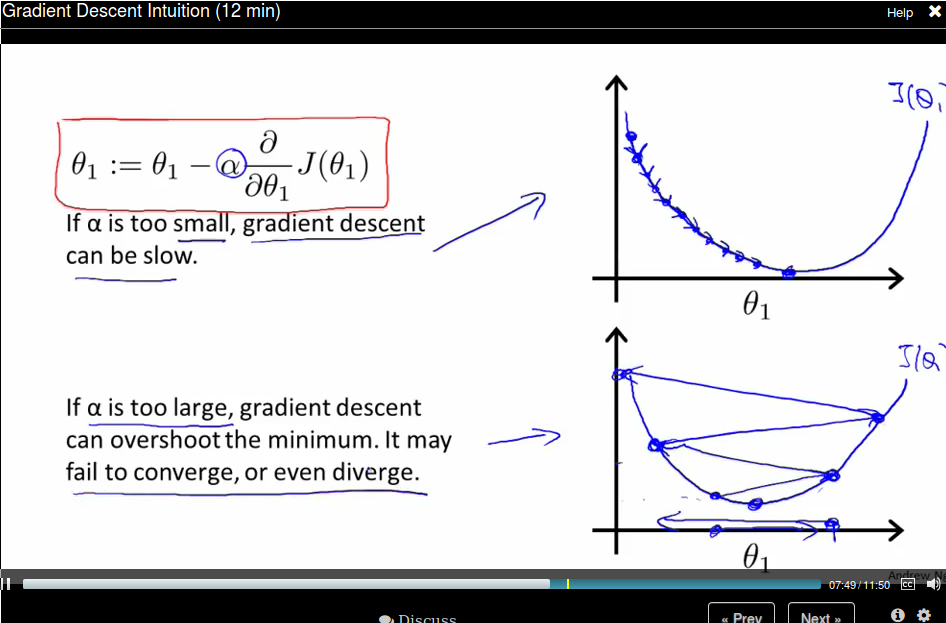
\includegraphics[width=.9\linewidth]{./images/screenshot-12.png}


Gradient descent can converge to a local minimum, even with the learning rate $\alpha$ fixed. This is because as we approach a local minimum, gradient descent will automatically take smaller steps. So no need to descrease $\alpha$ over time.


\textbf{Batch} Gradient descent:
Each step of gradient descent uses all the training examples:
\section*{Linear Algebra (Week1, Optional)}
\label{sec-4}
This lecture use 1-indexed subscripts.
\section*{Linear Regression with Multiple Variables (Week 2)}
\label{sec-5}
\subsection*{Multiple Features}
\label{sec-5-1}
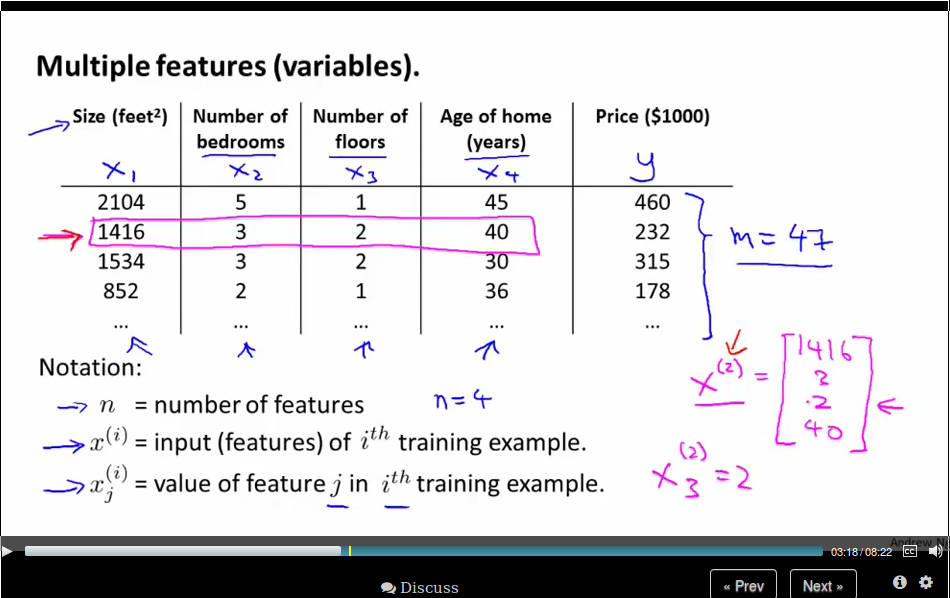
\includegraphics[width=.9\linewidth]{./images/screenshot-13.png}
Notation:
\begin{enumerate}
\item number of features: \(n\)
\item input (features) of \(i^{\text{th}}\) training example: \(x^{(i)}\)
\item value of feature \(j\) in \(i^{th}\) training example. \(x^{(i)}_{j}\)
\end{enumerate}

Now our hypothesis is \(h_\theta (x) = \theta_0 + \theta_1 x_1 +  \theta_2 x_2 + \dots + \theta_n x_n \).
For convenience of notation, define \(x_0 = 1\), or \(x^{(i)}_0 = 1\). So now we define our hypothesis as
\begin{equation*}
\begin{split}
h_\theta (x) &= \theta_0 x_0 + \theta_1 x_1 +  \theta_2 x_2 + \dots + \theta_n x_n \\
&= \theta x
\end{split}
\end{equation*}
where \(\theta\) is a \(n+1\) dimension vector.
\subsection*{Gradient Descent for Multiple Variables}
\label{sec-5-2}
So now our new algorithm becomes
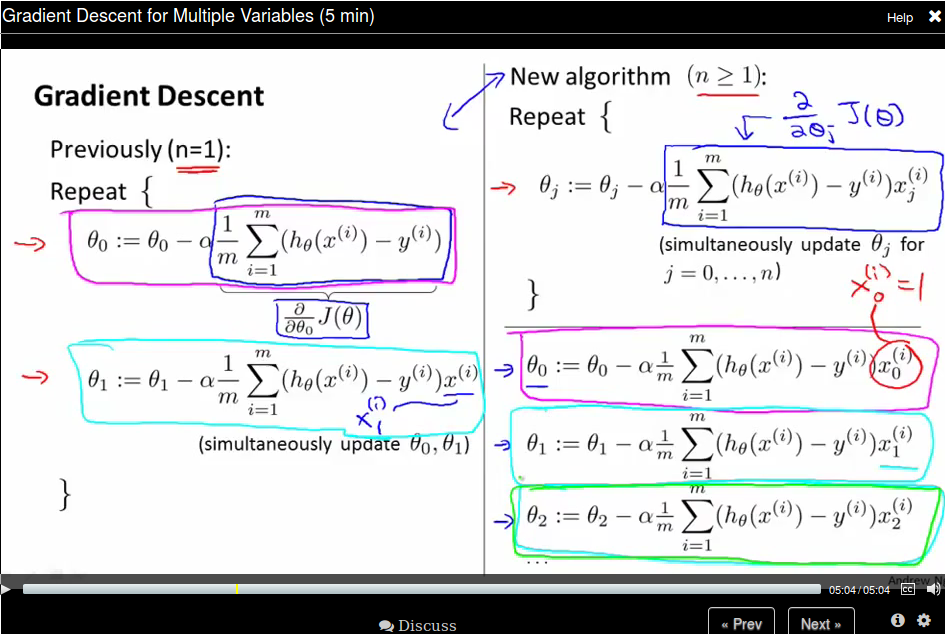
\includegraphics[width=.9\linewidth]{./images/screenshot-14.png}
Note that our new algorithm for $\theta_0$ is just like the old one since \(x_0^{(i)} \) is 1.
\subsection*{Gradient Descent in Practice - Feature Scaling.}
\label{sec-5-3}
Idea: Make sure features are on a similar scale, then gradient descent will converge more quickly.

Take a 2D example,  if the dimension of \(x_1\) is much larger than the dimension of \(x_2\), then the search region is a long ellipsis shape which is make gradient much difficult to find the minimum.
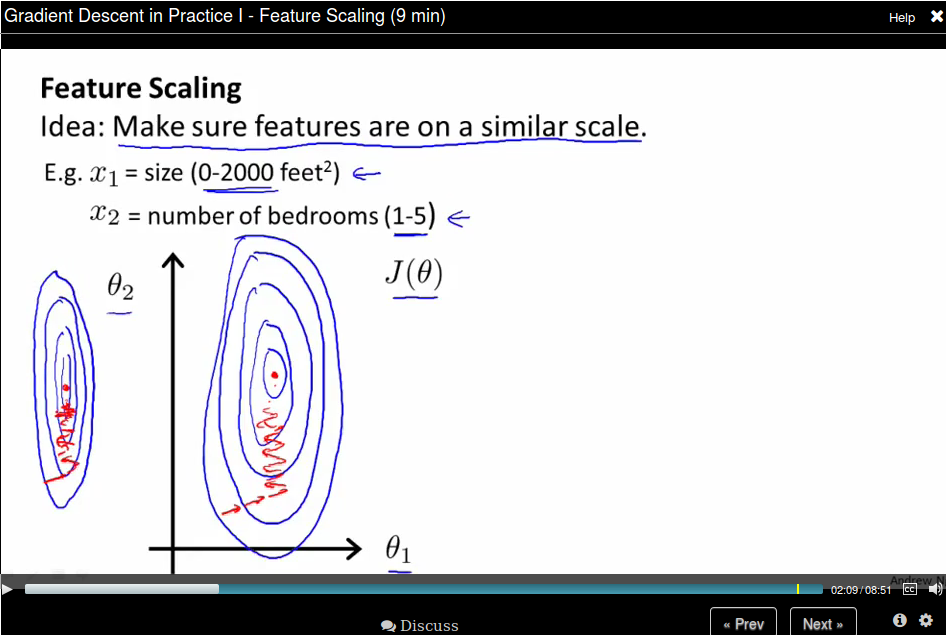
\includegraphics[width=.9\linewidth]{./images/screenshot-15.png}
We can rescale all features to [0,1] so the contours now become a circle.
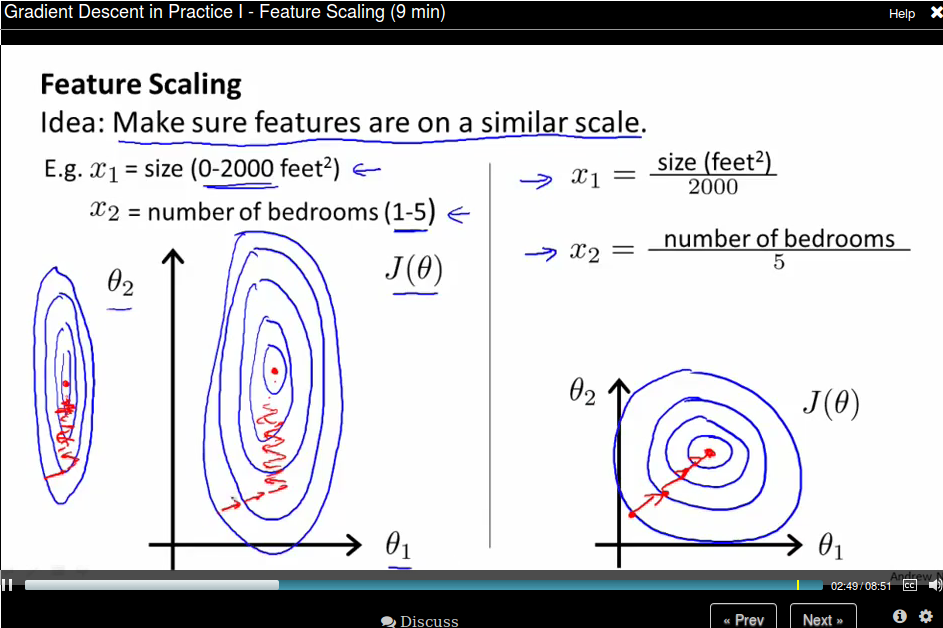
\includegraphics[width=.9\linewidth]{./images/screenshot-16.png}

Usually we get every feature into approximately a \(-1 \leq x \leq 1\) range. But it need not to be exactly. Say \(-3 \leq x \leq 3 \) is OK.


Mean normalization: Replace \(x_i\) with \(x_i - \mu_i\) to make features have approximately zero mean. Note that this does not apply to \(x_0 = 1\).
\subsection*{Gradient Descent in Practice - Learning Rate.}
\label{sec-5-4}
To make sure gradient descent is working correctly, draw the figure the value of \(J(\theta)\) versus the number of iterations.
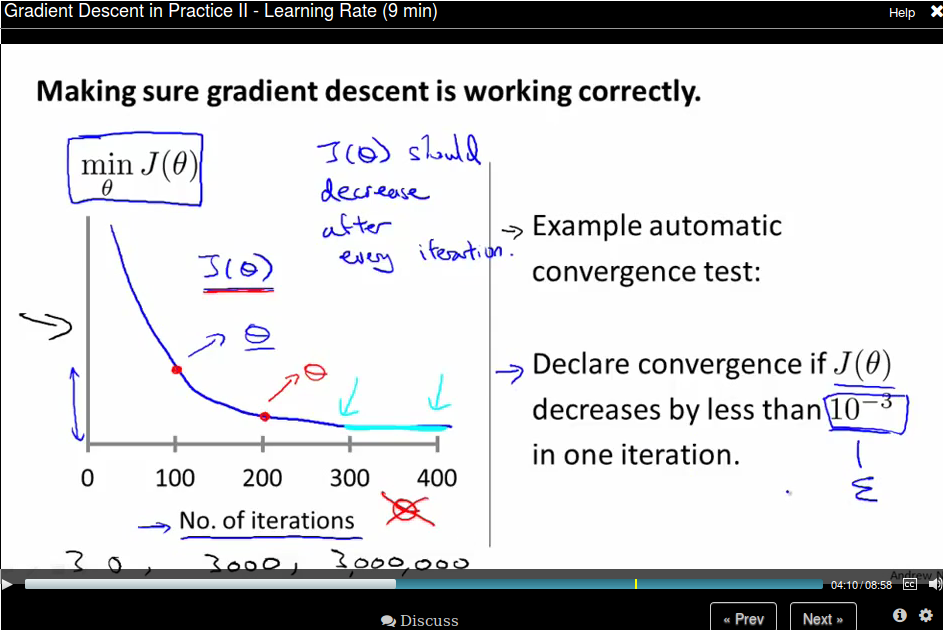
\includegraphics[width=.9\linewidth]{./images/screenshot-17.png}

For sufficiently small \(\alpha\), \(J(\theta\) should decrease on every iteration. But if $\alpha$  is too small, gradient descent can converge too slow. To choose \(\alpha\) try \( \dots, 0.001, 0.003,0.01, 0.03,0.1, 0.3,1, \dots\), roughly a 3x larger.
\subsection*{Features and Polynomial Regression}
\label{sec-5-5}
You need to choose a good feature instead of just using what you're provided. For example, for housing price prediction, you are provided with the frontage and depth feature, you can define a feature called area = frontage x depth.
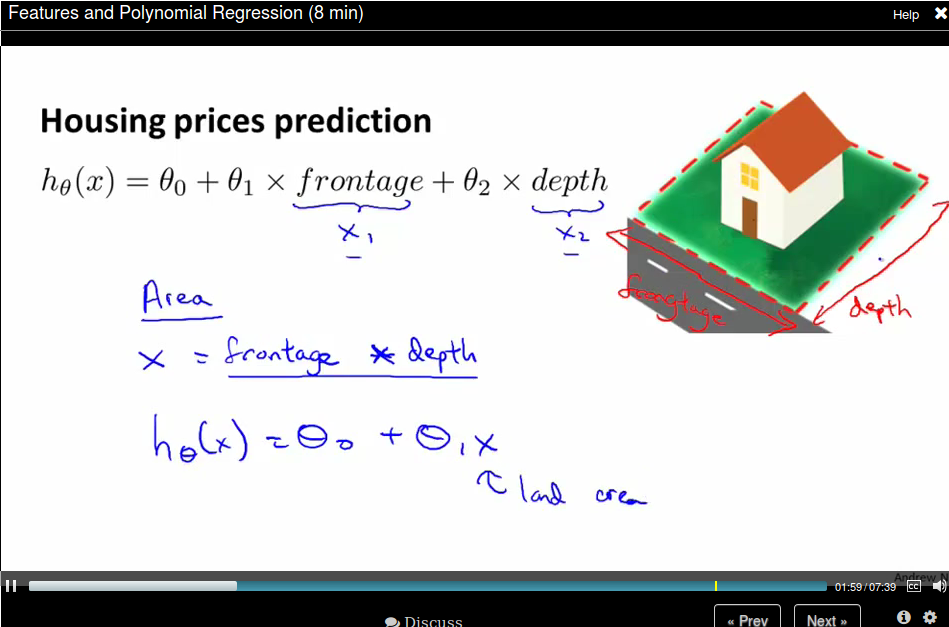
\includegraphics[width=.9\linewidth]{./images/screenshot-18.png}

Or sometimes use a polynomial function would be better. If the feature is not enough, you could use size, size\^{}2, size\^{}3 as features.
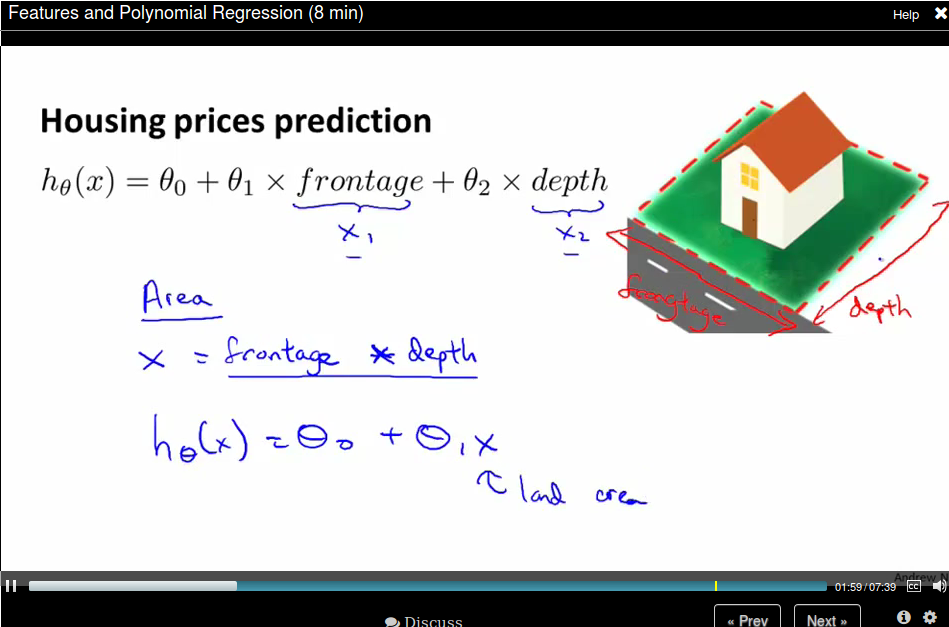
\includegraphics[width=.9\linewidth]{./images/screenshot-18.png}

Or you can use square root as feature.
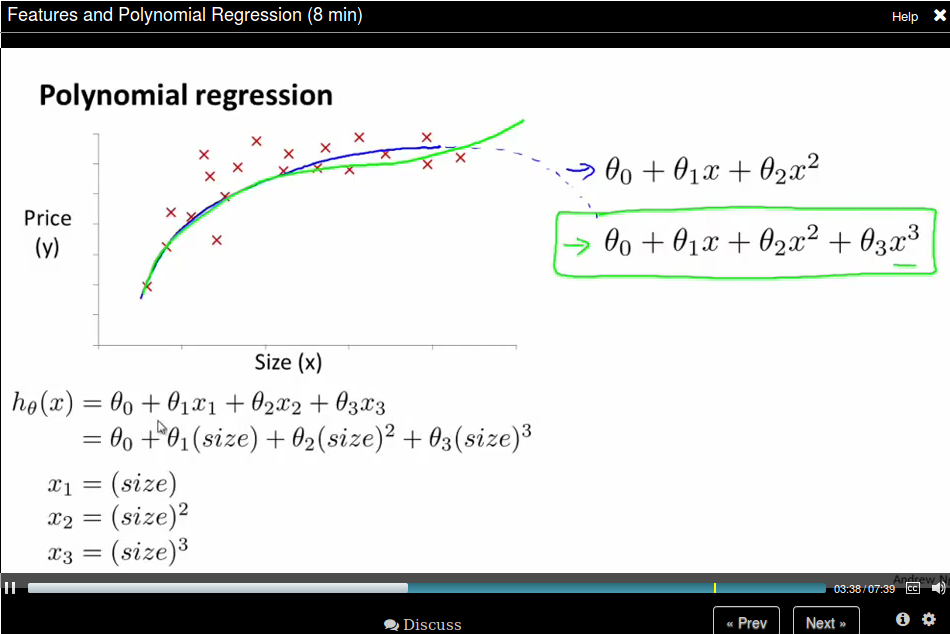
\includegraphics[width=.9\linewidth]{./images/screenshot-19.png}
How to find the minimum of \(J(\theta)\) analytically?

By Calculus, we can take the partial derivatives of each variable, and set it to 0.

Normal Equation:
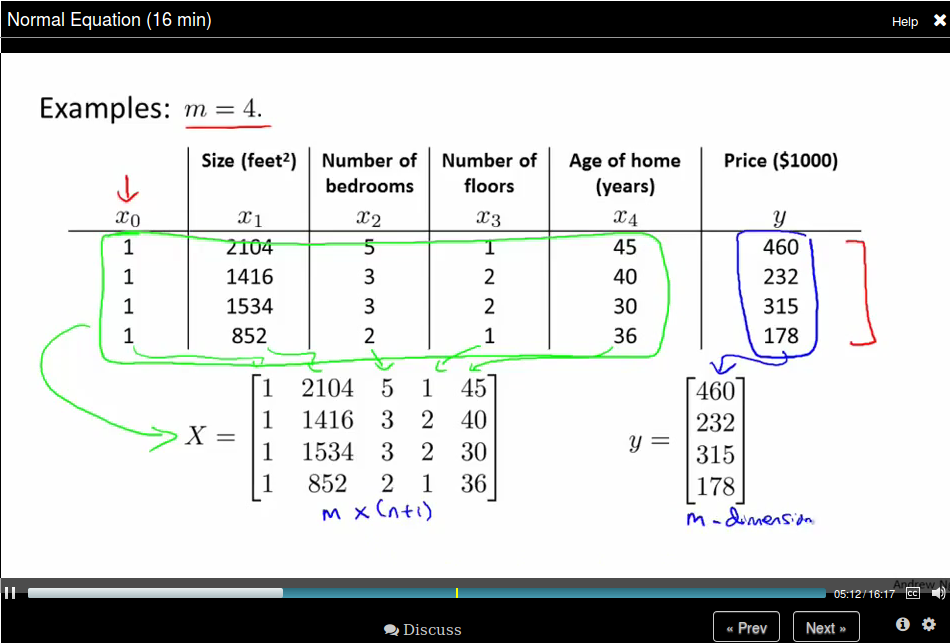
\includegraphics[width=.9\linewidth]{./images/screenshot-22.png}
Then we can compute $\theta = (X^T X)^{-1} X^T y$
The Octave code is:
\begin{minted}[]{octave}
pinv(X' * X) * X' * y
\end{minted}
Compare Gradient Descent with Normal Equation.
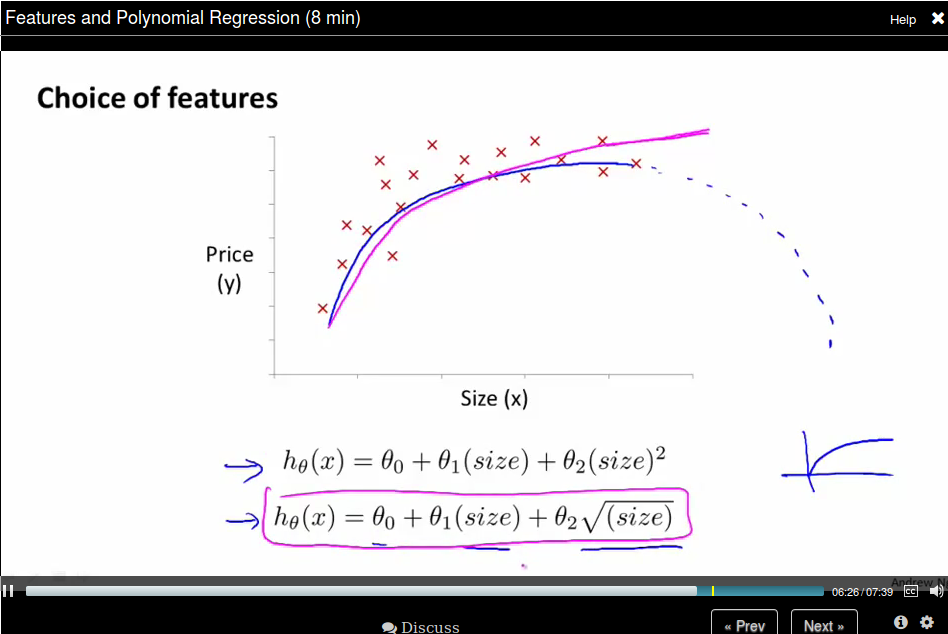
\includegraphics[width=.9\linewidth]{./images/screenshot-20.png}
\subsection*{Normal Equation and Noninvertbility (Optional)}
\label{sec-5-6}
Use \texttt{pinv} in Octave should not be a problem.
What if \(X^T X\) is non-invertible?
\begin{enumerate}
\item Reduent features (linearyly dependant).
E.g. $x_1$ = size in feet, $x_2$ size in m\^{}2.
\item Too many features (e.g. \$m $\le$ n).
Delete some features, or use regulariation.
\end{enumerate}



\section*{Octave Tutorial}
\label{sec-6}
\subsection*{Basic Operation}
\label{sec-6-1}
\begin{minted}[]{octave}
5+6
3-2
5*8
1/2
2^6


1 == 2 %false
1 ~= 2 
1 && 0
1 || 0

xor(1,0) %XOR

PS1('>> '); % to change the prompt sign

a = 3; % semicolon supressing output
a

disp(a);
disp(sprintf('2 decimals: %0.2f', a))

a
format long
a
format short
a

A = [1 2; 3 4; 5 6]

A = [1 2
     3 4
     5 6]

v = [1 2 3]

v = 1:0.1:2

ones(2,3)

C = 2*ones(2,3)

C = [2 2 2; 2 2 2]

w = ones(1,3)
w = zeros(1,3)
w = rand(1,3)

rand(3,3)
rand(3,3)

w = randn(1,3) % guassian distribution

w = -6 + sqrt(10)*(randn(1,10000)); % you don't want to omit the semicolon here

hist(w)
hist(w,50)

eye(4) % identity matrix
I = eye(6)

help eye
\end{minted}

\subsection*{Move data around}
\label{sec-6-2}
\begin{minted}[]{octave}
A = [1 2; 3 5; 5 6]
size(A)
sz = size(A)
size(A,1)
v = [1 2 3 4]
length(v)
length(A)
length([1;2;3;4;5])
pwd
cd ..
ls
load('test.dat')
who
whos
save hello.mat v
save hello.txt v -ascii
clear
A = [1 2 ; 3 4; 5 6];
A(3,2)
A(:,2)
A([1 3], :)
A(:,2) = [10; 11; 12]
A = [A, [ 100, 101, 102]];
A(:) % put all elements of A into a single vector
A = [1 2; 3 4; 5 7];
B = [11 12; 13 14; 15 16];
C = [A B]
C = [A,B]
D = [A; B]
\end{minted}
\subsection*{Computing on Data}
\label{sec-6-3}
\begin{minted}[]{octave}
A = [1 2; 3 4; 5 6];
B = [11 12; 13 14; 15 16];
C = [11 12; 13 14]

A.*B
A.^2
v = [1; 2; 3]
1 ./ v
1 ./ A
log(v)
exp(v)
abs(v)
abs([-1; 2; -3])
-v
v + ones(length(v),1)
v + 1

A'
(A')'

a = [1 15 2 0.5]
val = max(a)
[val, ind] = max(a)
max(A)
a < 3
A = magic(3)
[r,c] = find(A >= 7)

sum(a)
prod(a)
floor(a)
ceil(a)

max(A,[],1) % colomn wise max
max(A,[],2) % row wise max
max(A)
max(max(A))
max(A(:)) % find max of all the elements

A = magic(9)
sum(A,1) % column wise sum

sum(sum(A .* (eye(9)))) % sum the diagonal values
sum(sum(A .*flipud(eye(9)))) % sum the subdiagonal values

pinv(A)                         # sudo inverse
temp = pinv(A)
temp * A
\end{minted}
\subsection*{Plotting Data}
\label{sec-6-4}
\begin{minted}[]{octave}
t = [0:0.01:0.98];
y1 = sin(2*pi*4*t);
plot(t,y1);
y2 = cos(2*pi*4*t);
plot(t,y2);

plot(t,y1);
hold on;
plot(t,y2,'r');
xlabel('time');
ylabel('value');
legend('sin','cos');
title('my plot');
print -dpng 'myPlot.png'
close


figure(1); plot(t,y1);
figure(2); plot(t,y2);

subplot(1,2,1)% divides plot into a 1x2 grid, access first element
plot(t,y1);
subplot(1,2,2);
plot(t,y2);
axis([0.5 1 -1 1]) % change horizontal range to [0.5,1] and vertical to [-1,1]

A = magic(5)
imagesc(A)
imagesc(A), colorbar, colormap gray; % use comma for command chainning, for ouput, which is different from semicolon
\end{minted}
\subsection*{Control Statements}
\label{sec-6-5}
\begin{minted}[]{octave}
v = zeros(10,1)
for i = 1:10,
    v(i) = 2^i;
end;

i = 1;
while i <= 5,
      v(i) = 100;
end


i = 1;
while true,
      v(i) = 999;
      i = i + 1;
      if( i == 6),
        break;
      end;
end;
\end{minted}
\subsection*{Vectorizatrion}
\label{sec-6-6}

$h_\theta(x) = \sum_{j=0}^{n} \theta_j x_j = \theta^T x$
\begin{minted}[]{octave}
%unvectorized implemenetation
  predictaion = 0.0;
  for j = 1;n+1,
      prediction = prediction + theta(j) * x(j)
  end;
  %vectorized implementation
  prediction = thteta' * x;
\end{minted}

\section*{Logistic Regression (Week 3)}
\label{sec-7}
Applying linear regression to a classification problem is not a good idea.
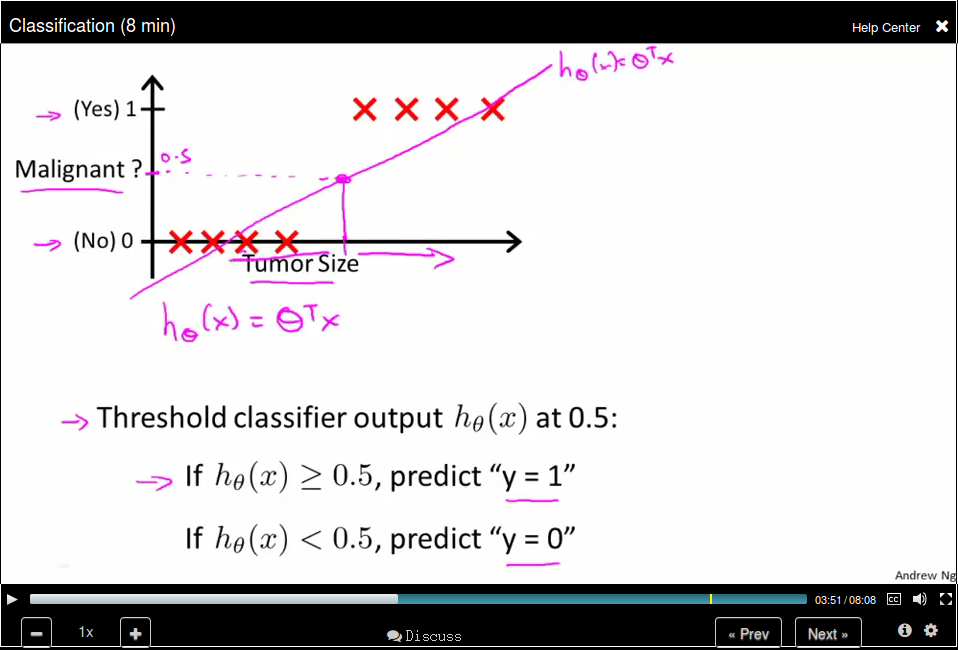
\includegraphics[width=.9\linewidth]{./images/screenshot-23.png}

You can use 0.5 as a threshhold to do the prediction based on the h\_\$$\backslash$theta\$(x)
value. However, this is not a good idea since when adding a new sample point,
the hypothesis will change. Besides, the return value for h\_\$$\backslash$theta\$(x) could be
not in the range [0, 1], thus making the prediction rather confusing. Logistic
Regression, though the word regression, is used to do the classification job and
the hypothesis can be guaranteed in the range [0,1].
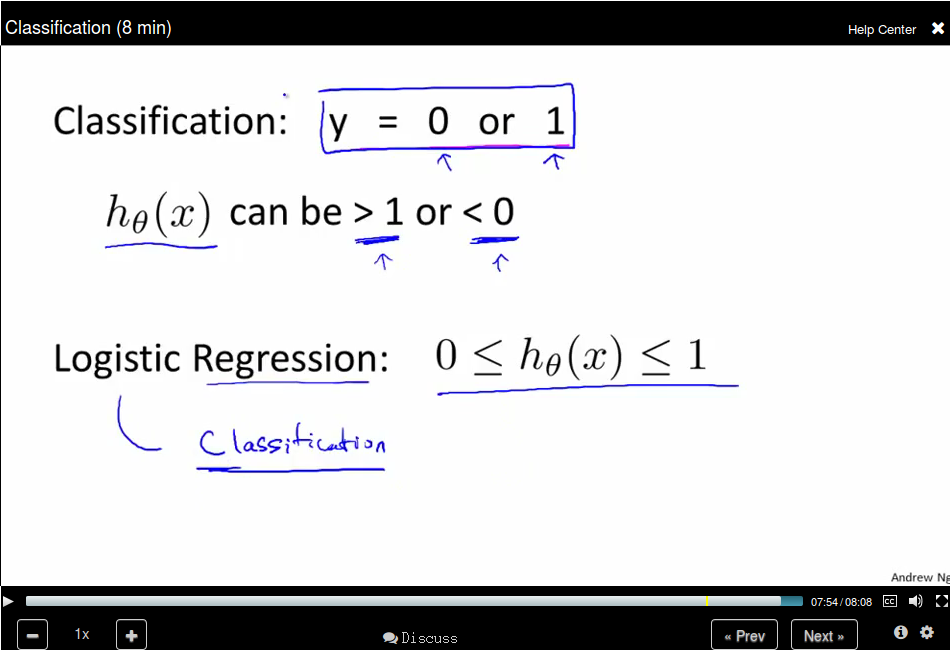
\includegraphics[width=.9\linewidth]{./images/screenshot-24.png}
% Emacs 24.4.1 (Org mode 8.2.10)
\end{document}